\section{手法の選定}
\label{sec_selection}
本章では，研究の初期に行った手法の比較を述べる．
この段階では，ラベルを単純な7クラスとし，ラベルの付け方そのものを比較した．

\subsection{初期のラベル}
初期のラベルは，ボケの生成の処理を決める形式と，事前知識の要否を決める画風の2つの軸で定義した．
形式は，主となる絵や写真がなく画像の大部分が文章である text，空欄の記号がある anaume，カルタの札の形式である karuta，それ以外の normal の4値とした．
画風は，写真 photo，アニメ anime，漫画 manga，その他の絵 illust の4値とした．
比較には，形式が normal 以外なら形式を，normal なら画風を採る7クラス（photo，anime，manga，text，anaume，karuta，illust）を用いた．
無作為抽出の440枚の目視ラベルでは，photo が44.5\%，anaume が22.3\%，illust が9.3\%，text が8.6\%，manga が7.0\%，anime が6.6\%，karuta が1.6\%であった．
穴埋めはお題の約4分の1を占め，最も多い特殊な形式である．

\subsection{比較した手法}
比較した手法は次の5系統である．
1つ目は，埋め込みモデルのゼロショット分類であり，各クラスに3個から4個の英語の文章を用意した．
2つ目は，メタデータを弱いラベルとした線形プローブである．
\texttt{type} 列とタグから各クラス1,500枚，計10,500枚を抽出し，その値をラベルとした．
3つ目は，Qwen3-VL の 2B，4B，8B の各モデルに，画像と2つの軸の定義を与えて直接分類させる方法である．
4つ目は，Qwen3-VL が10,500枚に付けたラベルで線形プローブを学習する蒸留である．
5つ目は，日本語の文字認識 (Optical Character Recognition，OCR) のライブラリ YomiToku\cite{ref_yomitoku} で文字の領域を検出し，文字の面積比と文字数が大きい画像を text とする規則である．
線形プローブは，標準化した埋め込みに対する L2 正則化付きのロジスティック回帰とした．

\subsection{初期の比較の結果}
図\ref{fig_speed_vs_f1}に，評価用データ440枚における各手法の処理速度と7クラスのマクロ F1 を示す．
横軸は1秒あたりの処理枚数，上側の横軸は全件の処理に要する時間であり，いずれも対数軸である．
図中の vlm は VLM による直接の分類，probe\_vlm は VLM のラベルによる蒸留，probe\_hand は目視ラベルによる線形プローブ，probe\_weak はメタデータの弱いラベルによる線形プローブ，zeroshot はゼロショット分類を表す．

\begin{figure}[t]
    \centering
    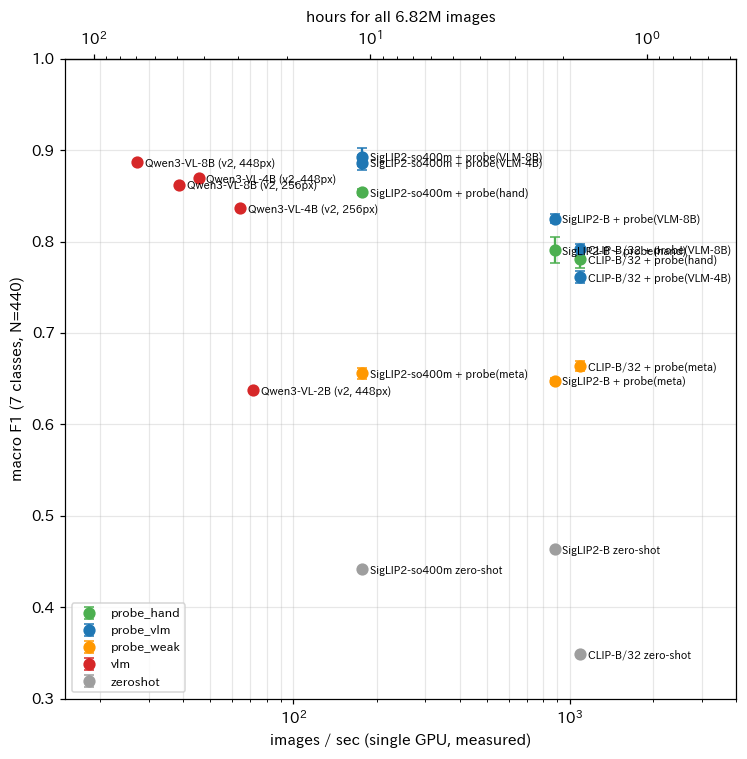
\includegraphics[width=\linewidth]{figures/fig_speed_vs_f1.png}
    \caption{初期のラベルにおける各手法の処理速度と7クラスのマクロ F1}
    \label{fig_speed_vs_f1}
\end{figure}

ゼロショット分類のマクロ F1 は 0.35 から 0.46 にとどまり，穴埋めの120枚のうち77枚を normal と予測した．
空欄があるという画像の部分的な特徴は，画像全体と文章の類似度では捉えにくい．
メタデータを弱いラベルとした学習は，正解率が約0.70にとどまった．
漫画のタグが付いた30枚のうち16枚が穴埋めであったように，メタデータは画像の種類と1対1に対応しないためである．
OCR の規則は，形式の正解率が 0.568 で，処理速度も毎秒6.4枚と遅かった．

Qwen3-VL-8B による直接の分類は正解率 0.905 であったが，処理速度は毎秒約27枚であり，全件に約70時間を要する．
このとき，プロンプトの text の定義を「画像の大部分が文章であり，主となる写真や絵がない」に限定し，字幕や看板を含む画像は normal とする記述を加えると，正解率は 0.718 から 0.905 に向上した．
限定する前のプロンプトでは，normal の219枚のうち98枚を text と予測していた．
モデルの大きさを変えるより，プロンプトの定義を明確にする効果の方が大きかった．

Qwen3-VL-8B のラベルで学習した SigLIP2-so400m の線形プローブは，正解率 0.913，マクロ F1 0.893 であり，教師と同等以上の精度を教師の約6.5倍の速度で得た．この生徒の速度は毎秒178枚であり，全件を約10.7時間で処理できる．
目視ラベル440枚で学習した線形プローブの正解率は 0.882 であり，VLM の約9,500枚のラベルによる学習に及ばなかった．
一方，教師を Qwen3-VL-2B にすると生徒の正解率は 0.726 にとどまり，教師の精度が生徒の精度の上限をおおむね決めていた．
これらの結果から，精度を決めるのはモデルの大きさよりもラベルの質であり，VLM の判断を高速な分類器に移す蒸留が有望であると判断した．

\subsection{蒸留の構成要素の比較}
次に，蒸留を構成する要素を1つずつ入れ替えて比較した．
この実験から，評価用データを640枚に拡充し，ハイパーパラメータを教師ラベルの検証用分割で選ぶようにした．
教師ラベル用の画像として，全てのお題から無作為に40,000枚を抽出し，学習用36,000枚と検証用4,000枚に分けた．
表\ref{tab_distill_components}に主な結果を示す．

\begin{table}[t]
    \centering
    \caption{蒸留の構成要素の比較（評価用データ640枚，7クラスの正解率）}
    \label{tab_distill_components}
    \small
    \begin{tabular}{lcc}
        \toprule
        手法 & 正解率 & 全件の時間 \\
        \midrule
        教師 Qwen3-VL-8B & 0.916 & 73 h \\
        教師 Qwen3-VL-32B（FP8） & 0.916 & 243 h \\
        教師 Qwen3-VL-30B-A3B（FP8） & 0.861 & 49 h \\
        教師 InternVL3.5-8B & 0.794 & 372 h \\
        教師 MiniCPM-V 4.5 & 0.684 & 143 h \\
        Qwen3-VL の3モデルの多数決 & 0.922 & -- \\
        \midrule
        LogReg，SigLIP2-so400m & 0.920 & 10.7 h \\
        MLP，SigLIP2-so400m & 0.911 & 10.7 h \\
        k 近傍法，SigLIP2-so400m & 0.811 & 10.7 h \\
        LogReg，SigLIP2-B & 0.867 & 2.2 h \\
        微調整 SigLIP2-B & 0.915 & 1.7 h \\
        微調整 ConvNeXt-Tiny & 0.902 & 2.7 h \\
        \bottomrule
    \end{tabular}
\end{table}

表\ref{tab_distill_components}の LogReg はロジスティック回帰，MLP は2層の多層パーセプトロン (Multi-Layer Perceptron，MLP) を表す．
生徒は全て Qwen3-VL-8B の教師ラベル36,000枚で学習し，3つの乱数の種の平均を示す．
教師は Qwen3-VL-8B が最良であった．
Qwen3-VL-32B は同じ正解率で約3.3倍遅く，30B-A3B と他系統の2モデルは穴埋めを過剰に検出する傾向があり，精度が劣った．
ただし，プロンプトは Qwen3-VL-8B の誤りを見て調整したものであり，他系統のモデルに不利な比較である可能性がある．
複数の教師の多数決は 8B 単体からの改善が0.6ポイントにとどまり，計算量に見合わなかった．

生徒では，ロジスティック回帰と MLP が同等であり，k 近傍法は件数の少ない karuta と雑多な illust で大きく劣った．
SigLIP2-B の微調整は，SigLIP2-B の埋め込みに対するロジスティック回帰より約5ポイント高く，SigLIP2-so400m の線形プローブと同等の精度を約6倍の速度で得た．
埋め込みの連結や，OpenCV で検出した空欄の矩形の特徴の追加による改善は0.005未満であり，強い埋め込みは空欄の情報を既に含んでいた．

図\ref{fig_learning_curve}に，教師ラベルの学習枚数と7クラスのマクロ F1 の関係を示す．
横軸は教師ラベルの学習枚数の対数，縦軸はマクロ F1 であり，実線は評価用データ，破線は教師ラベルの検証用分割での値である．
logreg はロジスティック回帰，mlp は MLP を表す．

\begin{figure}[t]
    \centering
    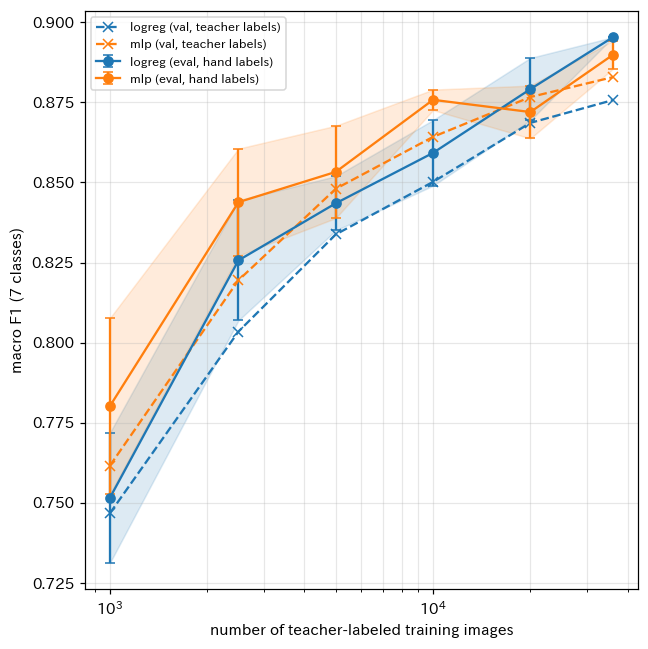
\includegraphics[width=0.9\linewidth]{figures/fig_learning_curve.png}
    \caption{教師ラベルの学習枚数とマクロ F1}
    \label{fig_learning_curve}
\end{figure}

マクロ F1 は学習枚数とともに単調に向上し，36,000枚でも飽和していなかった．
ロジスティック回帰の正解率は，1,000枚で 0.841，10,000枚で 0.891，36,000枚で 0.920 であった．
一方，メタデータで少ない種類を多めに抽出した9,450枚で学習した場合の正解率は 0.919 であり，無作為抽出の36,000枚と同等であった．
無作為抽出ではカルタが約1.3\%しか含まれないため，少ない種類を多めに含む画像に教師ラベルを付ける方が効率が良い．
この知見は，\ref{sec_student}章の少ない区分の追加につながった．

生徒の確信度が低い画像のみを VLM で判定し直すカスケードも比較した．
確信度は形式と画風の最大確率の積とした．
判定し直す割合が10\%から20\%のとき正解率は約1ポイント向上したが，全件の処理時間は約25時間に増え，改善の幅も次節で述べる目視ラベルの揺れと同程度であった．

\subsection{強い手法に共通する誤り}
Qwen3-VL-8B，SigLIP2-so400m の線形プローブ，微調整した SigLIP2-B の3手法が，互いに同じ予測をしたうえで目視ラベルと異なった画像は，640枚中23枚であった．
その多くは，文字を含む写真やイラストを text と予測したもの，空欄を含む文章を text と予測したものであった．
図\ref{fig_edge_text}に例を示す．
各画像の上の now は当時の目視ラベル，8B は Qwen3-VL-8B の予測，FT は微調整した SigLIP2-B の予測，proposal は後に提案した定義でのラベルを，「形式/画風」の形で示す．

\begin{figure}[t]
    \centering
    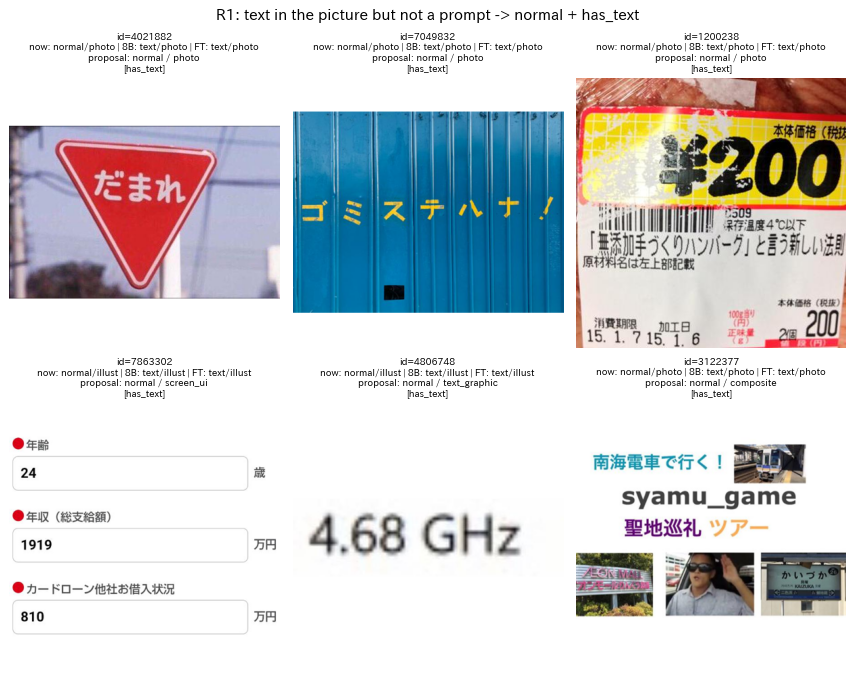
\includegraphics[width=\linewidth]{figures/fig_edge_text.png}
    \caption{文字を含むが回答者への問いではない画像の例}
    \label{fig_edge_text}
\end{figure}

標識，壁の文字，商品のラベル，入力フォームの画面は，目視では文章のお題ではないとして normal としたが，手法はいずれも text と予測した．
「画像の大部分が文章である」という見た目の基準では，これらの画像を text から除けない．
しかし，これらに必要なのは文章に答える処理ではなく，写真に一言を付ける通常の処理である．
以上から，約92\%の精度の上限は手法の差ではなくラベルの定義の曖昧さによって決まっていると判断し，ラベルの定義の見直しに進んだ．
